\documentclass[a4paper, 10pt]{article}
%\usepackage{fontspec}
%\setmainfont{Lato}
\usepackage{pgf}
\usepackage{eurosym}
\usepackage{graphicx}
\usepackage{wasysym}
\usepackage{hyperref}
\usepackage{listings}
\usepackage{pxfonts}
\usepackage{verbatim}
\usepackage{color}
\usepackage{xcolor}
\usepackage{wrapfig}
\usepackage{enumitem}
\usepackage{booktabs}
\usepackage{gensymb}
\usepackage{tabularx}
\usepackage{currfile}

\hypersetup{
    bookmarks=true,         % show bookmarks bar?
    unicode=true,          % non-Latin characters in Acrobat’s bookmarks
    pdftoolbar=true,        % show Acrobat’s toolbar?
    pdfmenubar=true,        % show Acrobat’s menu?
    pdffitwindow=true,     % window fit to page when opened
    pdftitle={Assessments},    % title
    pdfauthor={Paul Vesey},     % author
    pdfsubject={Advanced Graphics Assignment },   % subject of the document
    pdfcreator={},   % creator of the document
    pdfproducer={xelatex}, % producer of the document
    pdfkeywords={'Graphics' }, % list of keywords
    pdfnewwindow=true,      % links in new PDF window
    colorlinks=true,       % false: boxed links; true: colored links
    linkcolor=violet,          % color of internal links (change box color with linkbordercolor)
    citecolor=magenta,        % color of links to bibliography
    filecolor=red,      % color of file links
    urlcolor=blue           % color of external links
}

\setlength\parindent{0pt}
\begin{document}

\lstset{language=HTML,
				basicstyle=\small,
				breaklines=true,
        numbers=left,
        numberstyle=\tiny,
        showstringspaces=false,
        aboveskip=-20pt,
        frame=leftline
        }
				
\begin{table}%
	\begin{minipage}{0.4\textwidth}%
			
\includegraphics[width=1\textwidth]{./img/LITlogo.jpg}
	\end{minipage}
	\qquad
	\centering
	\parbox{0.4\textwidth}{
		\begin{large}			
			\begin{tabular}{| r | l |} \hline
				Subject: & \textbf{Advanced Graphics}\\
								 & \textbf{\& Visualisation}\\
				Course: & \textbf{Interior Design Y3}\\
				Session: & \textbf{Autumn 2020}\\
				Lecturer: & \textbf{Paul Vesey \footnotesize{BEng, MIE, HDip}}\\
				Filename: & \footnotesize{\currfilename}\\
				\hline
			\end{tabular}
		\end{large}			
	}
\end{table}
\vspace{0.25cm}	
	
\part*{Assignment 3 – Modern Residence with V-Ray }

\begin{tabularx}{\textwidth}{ |X|X| }
	\hline
	\textbf{Issue Date:} & 14$^{th}$ February 2019 \\
	\hline 
	\textbf{Submission Date:}  & As stated on Moodle  \\
	\hline
\end{tabularx}


\section*{Continuous Assessment Marks}
This assignment will account for 50\% of the 100\% allocated for continuous assessment in this module

\section*{Assignment Outline}
In this assignment you will create 5 high quality V-Ray renders from the Revit model provided.  The model has been sourced from  \href{https://enscape3d.com/free-sample-projects/}{https://enscape3d.com/free-sample-projects/} and has been upgraded to Revit 2019.\\

You are to create the following renders:

\begin{enumerate}
	\item External view of the building during daylight hours
	\item External view of the building in twilight, with artificial lights on.
	\item Internal view of your choice during daylight hours
	\item Internal view of your choice in twilight, with artificial lights on.
	\item Internal or External view of your choice.
\end{enumerate}

You have free reign to edit the materials used in the model as you see fit, however you must keep all model elements and their position as provided.\\

The following images are provided to illustrate the nature of the request.  Please note that these images were directly from the model and are fall far below the expected standard for this assignment. 


\begin{figure}[h]
	\centering
	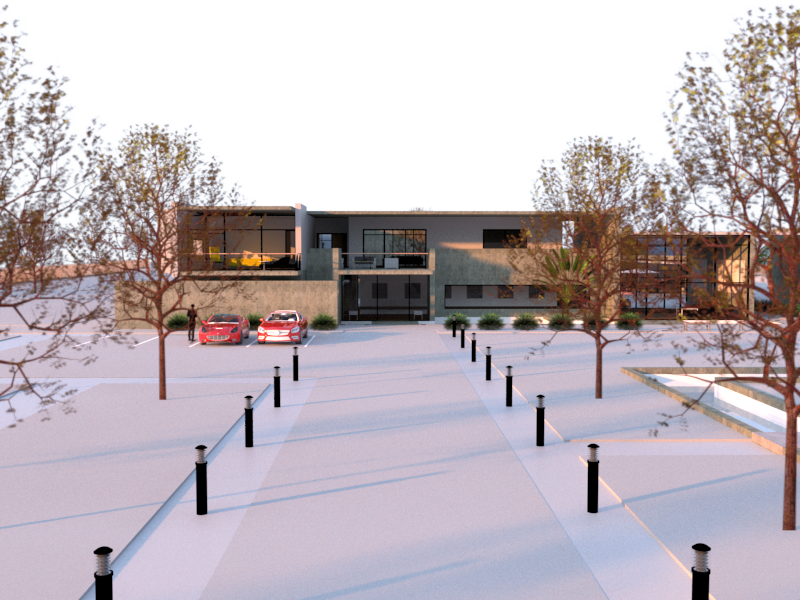
\includegraphics[width=1.0\linewidth]{img/Assignment3a}
	\caption{External View in Daylight}
	\label{fig:assignment3a}
\end{figure}


\begin{figure}[h]
	\centering
	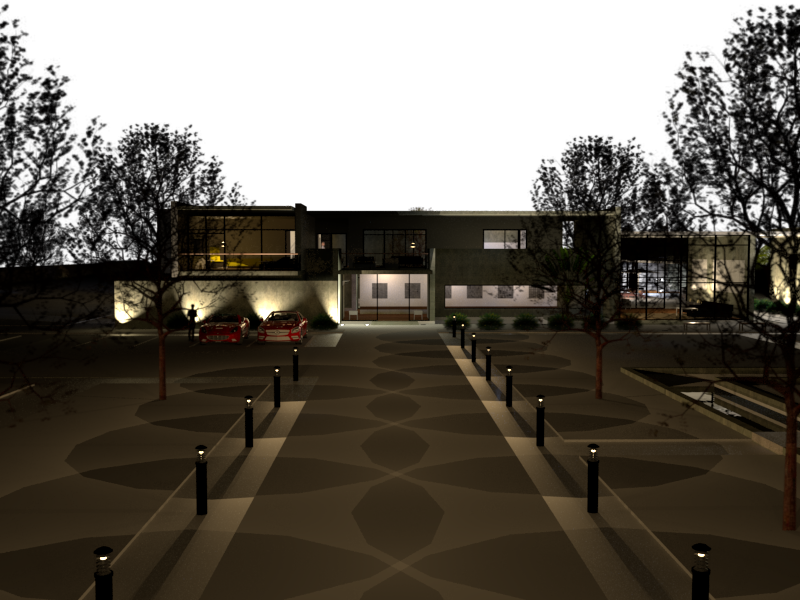
\includegraphics[width=1.0\linewidth]{img/Assignment3b}
	\caption{External View in Twilight.  (Note the sky is not shown)}
	\label{fig:assignment3b}
\end{figure}


\begin{figure}[h]
	\centering
	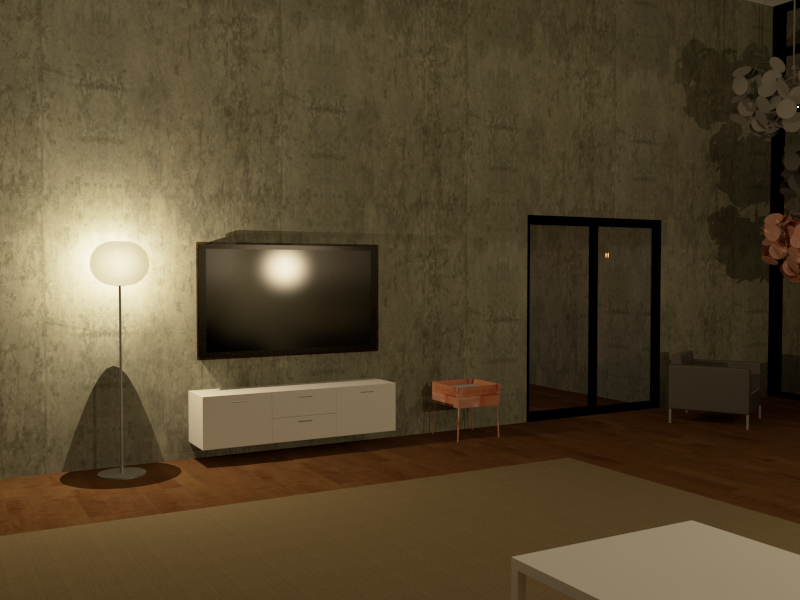
\includegraphics[width=1.0\linewidth]{img/Assignment3c}
	\caption{Internal View in Twilight.}
	\label{fig:assignment3c}
\end{figure}

\begin{figure}[h]
	\centering
	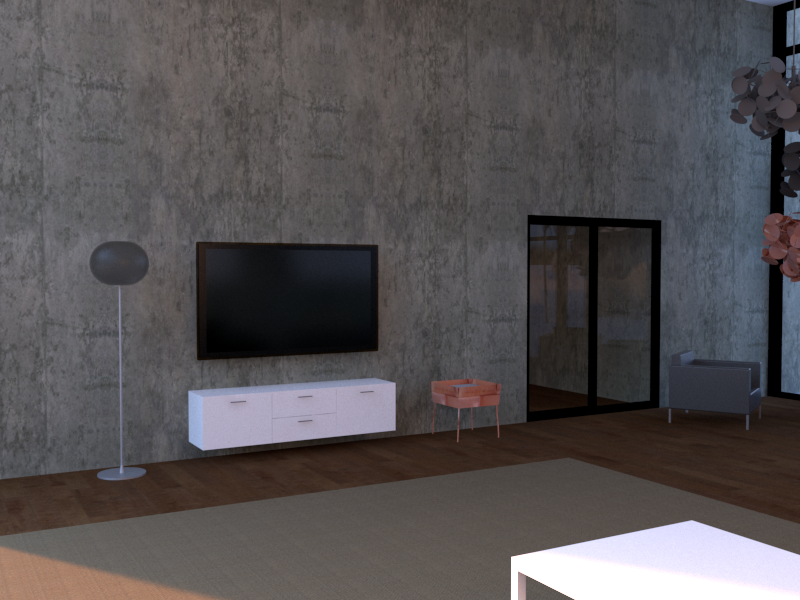
\includegraphics[width=1.0\linewidth]{img/Assignment3d}
	\caption{Internal View.}
	\label{fig:assignment3d}
\end{figure}




\newpage

\section*{Production Method}

You should make full use of the tools available to you for the production of these images.  These include the suite of tools available within Revit and V-Ray for materials, lighting, HDR, Image channels, and post production within Photoshop.\\

As part of this assignment you are required to submit a one page report on the production methodology used for each image.  This report should include details of the functionality used, exposure values, intensity values, atmospheric or any other effects used in V-Ray.  It should also detail the usage of Photoshop for compositing and any other modifications made. \\

An asset pack has been made available to you for this assignment.  The asset pack contains the following elements:

\begin{itemize}
	\item Revit Model sourced from \href{https://enscape3d.com/free-sample-projects/}{https://enscape3d.com/free-sample-projects/}
	\item HDRs for Lighting sourced from \href{https://hdrihaven.com/}{https://hdrihaven.com/}
	\item V-Ray RPC proxies are available on the lab machines
	\item V-Ray materials are available on the lab machines
	
\end{itemize}



\section*{Submission}
Upon completion, create a single zip file of your Revit model, render output, and all production files.  The files should be placed in a logical folder structure reflective of the file content and the production method.  You should also have one folder titled 'FinalRenders' where duplicates of your final images are placed.  Upload this single zip file to Moodle on or before the submission deadline.









\end{document}